% This file was created with tikzplotlib v0.10.1.
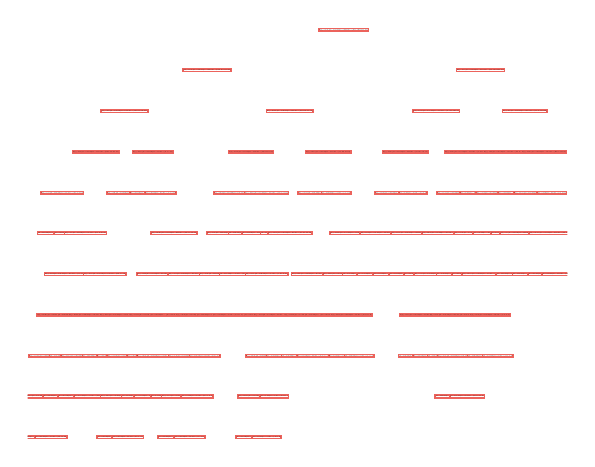
\begin{tikzpicture}

\definecolor{darkgray176}{RGB}{176,176,176}
\definecolor{tomato2369992}{RGB}{236,99,92}

\begin{axis}[
hide x axis,
hide y axis,
tick align=outside,
tick pos=left,
x grid style={darkgray176},
xmin=0, xmax=1,
xtick style={color=black},
y grid style={darkgray176},
ymin=0, ymax=1,
ytick style={color=black}
]
\draw (axis cs:0.0142857142857143,0.0454545454545455) node[
  scale=0.05,
  fill=white,
  draw=tomato2369992,
  line width=0.6pt,
  inner sep=3.6pt,
  text=black,
  rotate=0.0,
  align=center
]{gini = 0.339
samples = 688
value = [541, 3, 2, 142]};
\draw (axis cs:0.0428571428571429,0.0454545454545455) node[
  scale=0.05,
  fill=white,
  draw=tomato2369992,
  line width=0.6pt,
  inner sep=3.6pt,
  text=black,
  rotate=0.0,
  align=center
]{gini = 0.458
samples = 355
value = [230, 1, 0, 124]};
\draw (axis cs:0.157142857142857,0.0454545454545455) node[
  scale=0.05,
  fill=white,
  draw=tomato2369992,
  line width=0.6pt,
  inner sep=3.6pt,
  text=black,
  rotate=0.0,
  align=center
]{gini = 0.499
samples = 134
value = [75, 1, 0, 58]};
\draw (axis cs:0.185714285714286,0.0454545454545455) node[
  scale=0.05,
  fill=white,
  draw=tomato2369992,
  line width=0.6pt,
  inner sep=3.6pt,
  text=black,
  rotate=0.0,
  align=center
]{gini = 0.253
samples = 187
value = [160, 1, 3, 23]};
\draw (axis cs:0.271428571428571,0.0454545454545455) node[
  scale=0.05,
  fill=white,
  draw=tomato2369992,
  line width=0.6pt,
  inner sep=3.6pt,
  text=black,
  rotate=0.0,
  align=center
]{gini = 0.572
samples = 279
value = [165, 16, 26, 72]};
\draw (axis cs:0.3,0.0454545454545455) node[
  scale=0.05,
  fill=white,
  draw=tomato2369992,
  line width=0.6pt,
  inner sep=3.6pt,
  text=black,
  rotate=0.0,
  align=center
]{gini = 0.251
samples = 113
value = [97, 3, 1, 12]};
\draw (axis cs:0.414285714285714,0.0454545454545455) node[
  scale=0.05,
  fill=white,
  draw=tomato2369992,
  line width=0.6pt,
  inner sep=3.6pt,
  text=black,
  rotate=0.0,
  align=center
]{gini = 0.715
samples = 55
value = [20, 16, 6, 13]};
\draw (axis cs:0.442857142857143,0.0454545454545455) node[
  scale=0.05,
  fill=white,
  draw=tomato2369992,
  line width=0.6pt,
  inner sep=3.6pt,
  text=black,
  rotate=0.0,
  align=center
]{gini = 0.55
samples = 63
value = [6, 10, 7, 40]};
\draw (axis cs:0.0285714285714286,0.136363636363636) node[
  scale=0.05,
  fill=white,
  draw=tomato2369992,
  line width=0.6pt,
  inner sep=3.6pt,
  text=black,
  rotate=0.0,
  align=center
]{X[0] <= 294.135
gini = 0.389
samples = 1043
value = [771, 4, 2, 266]};
\draw (axis cs:0.0571428571428571,0.136363636363636) node[
  scale=0.05,
  fill=white,
  draw=tomato2369992,
  line width=0.6pt,
  inner sep=3.6pt,
  text=black,
  rotate=0.0,
  align=center
]{gini = 0.245
samples = 560
value = [480, 0, 0, 80]};
\draw (axis cs:0.0857142857142857,0.136363636363636) node[
  scale=0.05,
  fill=white,
  draw=tomato2369992,
  line width=0.6pt,
  inner sep=3.6pt,
  text=black,
  rotate=0.0,
  align=center
]{gini = 0.465
samples = 337
value = [213, 0, 0, 124]};
\draw (axis cs:0.114285714285714,0.136363636363636) node[
  scale=0.05,
  fill=white,
  draw=tomato2369992,
  line width=0.6pt,
  inner sep=3.6pt,
  text=black,
  rotate=0.0,
  align=center
]{gini = 0.368
samples = 358
value = [274, 4, 3, 77]};
\draw (axis cs:0.171428571428571,0.136363636363636) node[
  scale=0.05,
  fill=white,
  draw=tomato2369992,
  line width=0.6pt,
  inner sep=3.6pt,
  text=black,
  rotate=0.0,
  align=center
]{X[2] <= 704.98
gini = 0.4
samples = 321
value = [235, 2, 3, 81]};
\draw (axis cs:0.2,0.136363636363636) node[
  scale=0.05,
  fill=white,
  draw=tomato2369992,
  line width=0.6pt,
  inner sep=3.6pt,
  text=black,
  rotate=0.0,
  align=center
]{gini = 0.0
samples = 24
value = [24, 0, 0, 0]};
\draw (axis cs:0.228571428571429,0.136363636363636) node[
  scale=0.05,
  fill=white,
  draw=tomato2369992,
  line width=0.6pt,
  inner sep=3.6pt,
  text=black,
  rotate=0.0,
  align=center
]{gini = 0.693
samples = 375
value = [100, 19, 133, 123]};
\draw (axis cs:0.257142857142857,0.136363636363636) node[
  scale=0.05,
  fill=white,
  draw=tomato2369992,
  line width=0.6pt,
  inner sep=3.6pt,
  text=black,
  rotate=0.0,
  align=center
]{gini = 0.67
samples = 189
value = [86, 17, 29, 57]};
\draw (axis cs:0.285714285714286,0.136363636363636) node[
  scale=0.05,
  fill=white,
  draw=tomato2369992,
  line width=0.6pt,
  inner sep=3.6pt,
  text=black,
  rotate=0.0,
  align=center
]{X[2] <= 953.62
gini = 0.5
samples = 392
value = [262, 19, 27, 84]};
\draw (axis cs:0.314285714285714,0.136363636363636) node[
  scale=0.05,
  fill=white,
  draw=tomato2369992,
  line width=0.6pt,
  inner sep=3.6pt,
  text=black,
  rotate=0.0,
  align=center
]{gini = 0.63
samples = 292
value = [146, 35, 18, 93]};
\draw (axis cs:0.428571428571429,0.136363636363636) node[
  scale=0.05,
  fill=white,
  draw=tomato2369992,
  line width=0.6pt,
  inner sep=3.6pt,
  text=black,
  rotate=0.0,
  align=center
]{X[0] <= 285.035
gini = 0.689
samples = 118
value = [26, 26, 13, 53]};
\draw (axis cs:0.457142857142857,0.136363636363636) node[
  scale=0.05,
  fill=white,
  draw=tomato2369992,
  line width=0.6pt,
  inner sep=3.6pt,
  text=black,
  rotate=0.0,
  align=center
]{gini = 0.6
samples = 37
value = [20, 11, 1, 5]};
\draw (axis cs:0.785714285714286,0.136363636363636) node[
  scale=0.05,
  fill=white,
  draw=tomato2369992,
  line width=0.6pt,
  inner sep=3.6pt,
  text=black,
  rotate=0.0,
  align=center
]{gini = 0.437
samples = 337
value = [12, 246, 49, 30]};
\draw (axis cs:0.814285714285714,0.136363636363636) node[
  scale=0.05,
  fill=white,
  draw=tomato2369992,
  line width=0.6pt,
  inner sep=3.6pt,
  text=black,
  rotate=0.0,
  align=center
]{gini = 0.228
samples = 1434
value = [10, 1253, 126, 45]};
\draw (axis cs:0.0428571428571429,0.227272727272727) node[
  scale=0.05,
  fill=white,
  draw=tomato2369992,
  line width=0.6pt,
  inner sep=3.6pt,
  text=black,
  rotate=0.0,
  align=center
]{X[2] <= 463.705
gini = 0.344
samples = 1603
value = [1251, 4, 2, 346]};
\draw (axis cs:0.0714285714285714,0.227272727272727) node[
  scale=0.05,
  fill=white,
  draw=tomato2369992,
  line width=0.6pt,
  inner sep=3.6pt,
  text=black,
  rotate=0.0,
  align=center
]{gini = 0.195
samples = 1420
value = [1265, 4, 0, 151]};
\draw (axis cs:0.1,0.227272727272727) node[
  scale=0.05,
  fill=white,
  draw=tomato2369992,
  line width=0.6pt,
  inner sep=3.6pt,
  text=black,
  rotate=0.0,
  align=center
]{X[2] <= 422.66
gini = 0.425
samples = 695
value = [487, 4, 3, 201]};
\draw (axis cs:0.128571428571429,0.227272727272727) node[
  scale=0.05,
  fill=white,
  draw=tomato2369992,
  line width=0.6pt,
  inner sep=3.6pt,
  text=black,
  rotate=0.0,
  align=center
]{gini = 0.454
samples = 23
value = [8, 0, 0, 15]};
\draw (axis cs:0.157142857142857,0.227272727272727) node[
  scale=0.05,
  fill=white,
  draw=tomato2369992,
  line width=0.6pt,
  inner sep=3.6pt,
  text=black,
  rotate=0.0,
  align=center
]{gini = 0.143
samples = 285
value = [263, 1, 0, 21]};
\draw (axis cs:0.185714285714286,0.227272727272727) node[
  scale=0.05,
  fill=white,
  draw=tomato2369992,
  line width=0.6pt,
  inner sep=3.6pt,
  text=black,
  rotate=0.0,
  align=center
]{X[3] <= 571.345
gini = 0.381
samples = 345
value = [259, 2, 3, 81]};
\draw (axis cs:0.214285714285714,0.227272727272727) node[
  scale=0.05,
  fill=white,
  draw=tomato2369992,
  line width=0.6pt,
  inner sep=3.6pt,
  text=black,
  rotate=0.0,
  align=center
]{gini = 0.487
samples = 302
value = [205, 21, 11, 65]};
\draw (axis cs:0.242857142857143,0.227272727272727) node[
  scale=0.05,
  fill=white,
  draw=tomato2369992,
  line width=0.6pt,
  inner sep=3.6pt,
  text=black,
  rotate=0.0,
  align=center
]{X[2] <= 514.375
gini = 0.703
samples = 564
value = [186, 36, 162, 180]};
\draw (axis cs:0.3,0.227272727272727) node[
  scale=0.05,
  fill=white,
  draw=tomato2369992,
  line width=0.6pt,
  inner sep=3.6pt,
  text=black,
  rotate=0.0,
  align=center
]{X[1] <= 52.19
gini = 0.567
samples = 684
value = [408, 54, 45, 177]};
\draw (axis cs:0.328571428571429,0.227272727272727) node[
  scale=0.05,
  fill=white,
  draw=tomato2369992,
  line width=0.6pt,
  inner sep=3.6pt,
  text=black,
  rotate=0.0,
  align=center
]{gini = 0.146
samples = 141
value = [130, 8, 0, 3]};
\draw (axis cs:0.442857142857143,0.227272727272727) node[
  scale=0.05,
  fill=white,
  draw=tomato2369992,
  line width=0.6pt,
  inner sep=3.6pt,
  text=black,
  rotate=0.0,
  align=center
]{X[3] <= 127.345
gini = 0.707
samples = 155
value = [46, 37, 14, 58]};
\draw (axis cs:0.471428571428571,0.227272727272727) node[
  scale=0.05,
  fill=white,
  draw=tomato2369992,
  line width=0.6pt,
  inner sep=3.6pt,
  text=black,
  rotate=0.0,
  align=center
]{gini = 0.613
samples = 127
value = [17, 64, 3, 43]};
\draw (axis cs:0.5,0.227272727272727) node[
  scale=0.05,
  fill=white,
  draw=tomato2369992,
  line width=0.6pt,
  inner sep=3.6pt,
  text=black,
  rotate=0.0,
  align=center
]{gini = 0.642
samples = 192
value = [17, 16, 76, 83]};
\draw (axis cs:0.528571428571429,0.227272727272727) node[
  scale=0.05,
  fill=white,
  draw=tomato2369992,
  line width=0.6pt,
  inner sep=3.6pt,
  text=black,
  rotate=0.0,
  align=center
]{gini = 0.623
samples = 120
value = [10, 29, 16, 65]};
\draw (axis cs:0.585714285714286,0.227272727272727) node[
  scale=0.05,
  fill=white,
  draw=tomato2369992,
  line width=0.6pt,
  inner sep=3.6pt,
  text=black,
  rotate=0.0,
  align=center
]{gini = 0.7
samples = 89
value = [17, 20, 13, 39]};
\draw (axis cs:0.614285714285714,0.227272727272727) node[
  scale=0.05,
  fill=white,
  draw=tomato2369992,
  line width=0.6pt,
  inner sep=3.6pt,
  text=black,
  rotate=0.0,
  align=center
]{gini = 0.449
samples = 36
value = [26, 5, 2, 3]};
\draw (axis cs:0.714285714285714,0.227272727272727) node[
  scale=0.05,
  fill=white,
  draw=tomato2369992,
  line width=0.6pt,
  inner sep=3.6pt,
  text=black,
  rotate=0.0,
  align=center
]{gini = 0.547
samples = 49
value = [6, 31, 9, 3]};
\draw (axis cs:0.742857142857143,0.227272727272727) node[
  scale=0.05,
  fill=white,
  draw=tomato2369992,
  line width=0.6pt,
  inner sep=3.6pt,
  text=black,
  rotate=0.0,
  align=center
]{gini = 0.089
samples = 737
value = [6, 703, 19, 9]};
\draw (axis cs:0.771428571428571,0.227272727272727) node[
  scale=0.05,
  fill=white,
  draw=tomato2369992,
  line width=0.6pt,
  inner sep=3.6pt,
  text=black,
  rotate=0.0,
  align=center
]{gini = 0.446
samples = 521
value = [18, 375, 88, 40]};
\draw (axis cs:0.8,0.227272727272727) node[
  scale=0.05,
  fill=white,
  draw=tomato2369992,
  line width=0.6pt,
  inner sep=3.6pt,
  text=black,
  rotate=0.0,
  align=center
]{X[1] <= 603.85
gini = 0.272
samples = 1771
value = [22, 1499, 175, 75]};
\draw (axis cs:0.842857142857143,0.227272727272727) node[
  scale=0.05,
  fill=white,
  draw=tomato2369992,
  line width=0.6pt,
  inner sep=3.6pt,
  text=black,
  rotate=0.0,
  align=center
]{gini = 0.414
samples = 53
value = [1, 39, 11, 2]};
\draw (axis cs:0.871428571428571,0.227272727272727) node[
  scale=0.05,
  fill=white,
  draw=tomato2369992,
  line width=0.6pt,
  inner sep=3.6pt,
  text=black,
  rotate=0.0,
  align=center
]{gini = 0.652
samples = 58
value = [1, 18, 26, 13]};
\draw (axis cs:0.0571428571428571,0.318181818181818) node[
  scale=0.05,
  fill=white,
  draw=tomato2369992,
  line width=0.6pt,
  inner sep=3.6pt,
  text=black,
  rotate=0.0,
  align=center
]{X[3] <= 118.015
gini = 0.28
samples = 3023
value = [2516, 8, 2, 497]};
\draw (axis cs:0.0857142857142857,0.318181818181818) node[
  scale=0.05,
  fill=white,
  draw=tomato2369992,
  line width=0.6pt,
  inner sep=3.6pt,
  text=black,
  rotate=0.0,
  align=center
]{gini = 0.145
samples = 1215
value = [1120, 3, 2, 90]};
\draw (axis cs:0.114285714285714,0.318181818181818) node[
  scale=0.05,
  fill=white,
  draw=tomato2369992,
  line width=0.6pt,
  inner sep=3.6pt,
  text=black,
  rotate=0.0,
  align=center
]{X[0] <= 301.425
gini = 0.434
samples = 718
value = [495, 4, 3, 216]};
\draw (axis cs:0.171428571428571,0.318181818181818) node[
  scale=0.05,
  fill=white,
  draw=tomato2369992,
  line width=0.6pt,
  inner sep=3.6pt,
  text=black,
  rotate=0.0,
  align=center
]{X[2] <= 408.19
gini = 0.287
samples = 630
value = [522, 3, 3, 102]};
\draw (axis cs:0.228571428571429,0.318181818181818) node[
  scale=0.05,
  fill=white,
  draw=tomato2369992,
  line width=0.6pt,
  inner sep=3.6pt,
  text=black,
  rotate=0.0,
  align=center
]{X[2] <= 231.395
gini = 0.672
samples = 866
value = [391, 57, 173, 245]};
\draw (axis cs:0.257142857142857,0.318181818181818) node[
  scale=0.05,
  fill=white,
  draw=tomato2369992,
  line width=0.6pt,
  inner sep=3.6pt,
  text=black,
  rotate=0.0,
  align=center
]{gini = 0.433
samples = 349
value = [255, 23, 13, 58]};
\draw (axis cs:0.285714285714286,0.318181818181818) node[
  scale=0.05,
  fill=white,
  draw=tomato2369992,
  line width=0.6pt,
  inner sep=3.6pt,
  text=black,
  rotate=0.0,
  align=center
]{gini = 0.216
samples = 364
value = [321, 24, 1, 18]};
\draw (axis cs:0.314285714285714,0.318181818181818) node[
  scale=0.05,
  fill=white,
  draw=tomato2369992,
  line width=0.6pt,
  inner sep=3.6pt,
  text=black,
  rotate=0.0,
  align=center
]{X[3] <= 582.81
gini = 0.519
samples = 825
value = [538, 62, 45, 180]};
\draw (axis cs:0.342857142857143,0.318181818181818) node[
  scale=0.05,
  fill=white,
  draw=tomato2369992,
  line width=0.6pt,
  inner sep=3.6pt,
  text=black,
  rotate=0.0,
  align=center
]{gini = 0.447
samples = 497
value = [343, 137, 8, 9]};
\draw (axis cs:0.371428571428571,0.318181818181818) node[
  scale=0.05,
  fill=white,
  draw=tomato2369992,
  line width=0.6pt,
  inner sep=3.6pt,
  text=black,
  rotate=0.0,
  align=center
]{gini = 0.621
samples = 97
value = [50, 21, 1, 25]};
\draw (axis cs:0.428571428571429,0.318181818181818) node[
  scale=0.05,
  fill=white,
  draw=tomato2369992,
  line width=0.6pt,
  inner sep=3.6pt,
  text=black,
  rotate=0.0,
  align=center
]{gini = 0.607
samples = 53
value = [30, 12, 6, 5]};
\draw (axis cs:0.457142857142857,0.318181818181818) node[
  scale=0.05,
  fill=white,
  draw=tomato2369992,
  line width=0.6pt,
  inner sep=3.6pt,
  text=black,
  rotate=0.0,
  align=center
]{X[1] <= 258.71
gini = 0.69
samples = 282
value = [63, 101, 17, 101]};
\draw (axis cs:0.514285714285714,0.318181818181818) node[
  scale=0.05,
  fill=white,
  draw=tomato2369992,
  line width=0.6pt,
  inner sep=3.6pt,
  text=black,
  rotate=0.0,
  align=center
]{X[3] <= 114.175
gini = 0.66
samples = 312
value = [27, 45, 92, 148]};
\draw (axis cs:0.542857142857143,0.318181818181818) node[
  scale=0.05,
  fill=white,
  draw=tomato2369992,
  line width=0.6pt,
  inner sep=3.6pt,
  text=black,
  rotate=0.0,
  align=center
]{gini = 0.726
samples = 101
value = [37, 23, 15, 26]};
\draw (axis cs:0.571428571428571,0.318181818181818) node[
  scale=0.05,
  fill=white,
  draw=tomato2369992,
  line width=0.6pt,
  inner sep=3.6pt,
  text=black,
  rotate=0.0,
  align=center
]{gini = 0.475
samples = 235
value = [160, 56, 3, 16]};
\draw (axis cs:0.6,0.318181818181818) node[
  scale=0.05,
  fill=white,
  draw=tomato2369992,
  line width=0.6pt,
  inner sep=3.6pt,
  text=black,
  rotate=0.0,
  align=center
]{X[3] <= 482.05
gini = 0.714
samples = 125
value = [43, 25, 15, 42]};
\draw (axis cs:0.728571428571429,0.318181818181818) node[
  scale=0.05,
  fill=white,
  draw=tomato2369992,
  line width=0.6pt,
  inner sep=3.6pt,
  text=black,
  rotate=0.0,
  align=center
]{X[1] <= 579.75
gini = 0.126
samples = 786
value = [12, 734, 28, 12]};
\draw (axis cs:0.785714285714286,0.318181818181818) node[
  scale=0.05,
  fill=white,
  draw=tomato2369992,
  line width=0.6pt,
  inner sep=3.6pt,
  text=black,
  rotate=0.0,
  align=center
]{X[0] <= 277.26
gini = 0.315
samples = 2292
value = [40, 1874, 263, 115]};
\draw (axis cs:0.828571428571429,0.318181818181818) node[
  scale=0.05,
  fill=white,
  draw=tomato2369992,
  line width=0.6pt,
  inner sep=3.6pt,
  text=black,
  rotate=0.0,
  align=center
]{gini = 0.625
samples = 84
value = [5, 20, 45, 14]};
\draw (axis cs:0.857142857142857,0.318181818181818) node[
  scale=0.05,
  fill=white,
  draw=tomato2369992,
  line width=0.6pt,
  inner sep=3.6pt,
  text=black,
  rotate=0.0,
  align=center
]{X[1] <= 776.08
gini = 0.607
samples = 111
value = [2, 57, 37, 15]};
\draw (axis cs:0.0714285714285714,0.409090909090909) node[
  scale=0.05,
  fill=white,
  draw=tomato2369992,
  line width=0.6pt,
  inner sep=3.6pt,
  text=black,
  rotate=0.0,
  align=center
]{X[2] <= 787.24
gini = 0.245
samples = 4238
value = [3636, 11, 4, 587]};
\draw (axis cs:0.142857142857143,0.409090909090909) node[
  scale=0.05,
  fill=white,
  draw=tomato2369992,
  line width=0.6pt,
  inner sep=3.6pt,
  text=black,
  rotate=0.0,
  align=center
]{X[3] <= 126.93
gini = 0.375
samples = 1348
value = [1017, 7, 6, 318]};
\draw (axis cs:0.242857142857143,0.409090909090909) node[
  scale=0.05,
  fill=white,
  draw=tomato2369992,
  line width=0.6pt,
  inner sep=3.6pt,
  text=black,
  rotate=0.0,
  align=center
]{X[2] <= 690.02
gini = 0.627
samples = 1215
value = [646, 80, 186, 303]};
\draw (axis cs:0.3,0.409090909090909) node[
  scale=0.05,
  fill=white,
  draw=tomato2369992,
  line width=0.6pt,
  inner sep=3.6pt,
  text=black,
  rotate=0.0,
  align=center
]{X[2] <= 383.8
gini = 0.444
samples = 1189
value = [859, 86, 46, 198]};
\draw (axis cs:0.357142857142857,0.409090909090909) node[
  scale=0.05,
  fill=white,
  draw=tomato2369992,
  line width=0.6pt,
  inner sep=3.6pt,
  text=black,
  rotate=0.0,
  align=center
]{X[2] <= 25.205
gini = 0.488
samples = 594
value = [393, 158, 9, 34]};
\draw (axis cs:0.385714285714286,0.409090909090909) node[
  scale=0.05,
  fill=white,
  draw=tomato2369992,
  line width=0.6pt,
  inner sep=3.6pt,
  text=black,
  rotate=0.0,
  align=center
]{gini = 0.355
samples = 660
value = [520, 98, 11, 31]};
\draw (axis cs:0.442857142857143,0.409090909090909) node[
  scale=0.05,
  fill=white,
  draw=tomato2369992,
  line width=0.6pt,
  inner sep=3.6pt,
  text=black,
  rotate=0.0,
  align=center
]{X[0] <= 282.56
gini = 0.704
samples = 335
value = [93, 113, 23, 106]};
\draw (axis cs:0.528571428571429,0.409090909090909) node[
  scale=0.05,
  fill=white,
  draw=tomato2369992,
  line width=0.6pt,
  inner sep=3.6pt,
  text=black,
  rotate=0.0,
  align=center
]{X[2] <= 670.46
gini = 0.704
samples = 413
value = [64, 68, 107, 174]};
\draw (axis cs:0.585714285714286,0.409090909090909) node[
  scale=0.05,
  fill=white,
  draw=tomato2369992,
  line width=0.6pt,
  inner sep=3.6pt,
  text=black,
  rotate=0.0,
  align=center
]{X[2] <= 446.43
gini = 0.603
samples = 360
value = [203, 81, 18, 58]};
\draw (axis cs:0.614285714285714,0.409090909090909) node[
  scale=0.05,
  fill=white,
  draw=tomato2369992,
  line width=0.6pt,
  inner sep=3.6pt,
  text=black,
  rotate=0.0,
  align=center
]{gini = 0.629
samples = 331
value = [140, 140, 17, 34]};
\draw (axis cs:0.642857142857143,0.409090909090909) node[
  scale=0.05,
  fill=white,
  draw=tomato2369992,
  line width=0.6pt,
  inner sep=3.6pt,
  text=black,
  rotate=0.0,
  align=center
]{gini = 0.697
samples = 1049
value = [336, 395, 243, 75]};
\draw (axis cs:0.671428571428571,0.409090909090909) node[
  scale=0.05,
  fill=white,
  draw=tomato2369992,
  line width=0.6pt,
  inner sep=3.6pt,
  text=black,
  rotate=0.0,
  align=center
]{gini = 0.657
samples = 879
value = [168, 431, 218, 62]};
\draw (axis cs:0.7,0.409090909090909) node[
  scale=0.05,
  fill=white,
  draw=tomato2369992,
  line width=0.6pt,
  inner sep=3.6pt,
  text=black,
  rotate=0.0,
  align=center
]{gini = 0.677
samples = 332
value = [9, 85, 120, 118]};
\draw (axis cs:0.728571428571429,0.409090909090909) node[
  scale=0.05,
  fill=white,
  draw=tomato2369992,
  line width=0.6pt,
  inner sep=3.6pt,
  text=black,
  rotate=0.0,
  align=center
]{gini = 0.717
samples = 412
value = [102, 158, 100, 52]};
\draw (axis cs:0.757142857142857,0.409090909090909) node[
  scale=0.05,
  fill=white,
  draw=tomato2369992,
  line width=0.6pt,
  inner sep=3.6pt,
  text=black,
  rotate=0.0,
  align=center
]{X[3] <= 36.89
gini = 0.271
samples = 3078
value = [52, 2608, 291, 127]};
\draw (axis cs:0.785714285714286,0.409090909090909) node[
  scale=0.05,
  fill=white,
  draw=tomato2369992,
  line width=0.6pt,
  inner sep=3.6pt,
  text=black,
  rotate=0.0,
  align=center
]{gini = 0.631
samples = 80
value = [0, 29, 36, 15]};
\draw (axis cs:0.814285714285714,0.409090909090909) node[
  scale=0.05,
  fill=white,
  draw=tomato2369992,
  line width=0.6pt,
  inner sep=3.6pt,
  text=black,
  rotate=0.0,
  align=center
]{gini = 0.452
samples = 106
value = [2, 75, 22, 7]};
\draw (axis cs:0.842857142857143,0.409090909090909) node[
  scale=0.05,
  fill=white,
  draw=tomato2369992,
  line width=0.6pt,
  inner sep=3.6pt,
  text=black,
  rotate=0.0,
  align=center
]{X[0] <= 277.535
gini = 0.644
samples = 195
value = [7, 77, 82, 29]};
\draw (axis cs:0.9,0.409090909090909) node[
  scale=0.05,
  fill=white,
  draw=tomato2369992,
  line width=0.6pt,
  inner sep=3.6pt,
  text=black,
  rotate=0.0,
  align=center
]{gini = 0.168
samples = 2207
value = [63, 1, 2008, 135]};
\draw (axis cs:0.928571428571429,0.409090909090909) node[
  scale=0.05,
  fill=white,
  draw=tomato2369992,
  line width=0.6pt,
  inner sep=3.6pt,
  text=black,
  rotate=0.0,
  align=center
]{gini = 0.291
samples = 737
value = [17, 1, 611, 108]};
\draw (axis cs:0.957142857142857,0.409090909090909) node[
  scale=0.05,
  fill=white,
  draw=tomato2369992,
  line width=0.6pt,
  inner sep=3.6pt,
  text=black,
  rotate=0.0,
  align=center
]{gini = 0.486
samples = 487
value = [30, 48, 337, 72]};
\draw (axis cs:0.985714285714286,0.409090909090909) node[
  scale=0.05,
  fill=white,
  draw=tomato2369992,
  line width=0.6pt,
  inner sep=3.6pt,
  text=black,
  rotate=0.0,
  align=center
]{gini = 0.312
samples = 3774
value = [294, 25, 3096, 359]};
\draw (axis cs:0.05,0.5) node[
  scale=0.05,
  fill=white,
  draw=tomato2369992,
  line width=0.6pt,
  inner sep=3.6pt,
  text=black,
  rotate=0.0,
  align=center
]{gini = 0.059
samples = 5026
value = [4873, 15, 0, 138]};
\draw (axis cs:0.0785714285714286,0.5) node[
  scale=0.05,
  fill=white,
  draw=tomato2369992,
  line width=0.6pt,
  inner sep=3.6pt,
  text=black,
  rotate=0.0,
  align=center
]{gini = 0.271
samples = 303
value = [256, 35, 0, 12]};
\draw (axis cs:0.107142857142857,0.5) node[
  scale=0.05,
  fill=white,
  draw=tomato2369992,
  line width=0.6pt,
  inner sep=3.6pt,
  text=black,
  rotate=0.0,
  align=center
]{X[5] <= 52.5
gini = 0.28
samples = 5586
value = [4653, 18, 10, 905]};
\draw (axis cs:0.271428571428571,0.5) node[
  scale=0.05,
  fill=white,
  draw=tomato2369992,
  line width=0.6pt,
  inner sep=3.6pt,
  text=black,
  rotate=0.0,
  align=center
]{X[3] <= 145.415
gini = 0.551
samples = 2404
value = [1505, 166, 232, 501]};
\draw (axis cs:0.371428571428571,0.5) node[
  scale=0.05,
  fill=white,
  draw=tomato2369992,
  line width=0.6pt,
  inner sep=3.6pt,
  text=black,
  rotate=0.0,
  align=center
]{X[3] <= 58.75
gini = 0.425
samples = 1254
value = [913, 256, 20, 65]};
\draw (axis cs:0.4,0.5) node[
  scale=0.05,
  fill=white,
  draw=tomato2369992,
  line width=0.6pt,
  inner sep=3.6pt,
  text=black,
  rotate=0.0,
  align=center
]{gini = 0.445
samples = 52
value = [11, 3, 1, 37]};
\draw (axis cs:0.428571428571429,0.5) node[
  scale=0.05,
  fill=white,
  draw=tomato2369992,
  line width=0.6pt,
  inner sep=3.6pt,
  text=black,
  rotate=0.0,
  align=center
]{gini = 0.584
samples = 1314
value = [624, 565, 38, 87]};
\draw (axis cs:0.457142857142857,0.5) node[
  scale=0.05,
  fill=white,
  draw=tomato2369992,
  line width=0.6pt,
  inner sep=3.6pt,
  text=black,
  rotate=0.0,
  align=center
]{gini = 0.0
samples = 24
value = [0, 0, 0, 24]};
\draw (axis cs:0.485714285714286,0.5) node[
  scale=0.05,
  fill=white,
  draw=tomato2369992,
  line width=0.6pt,
  inner sep=3.6pt,
  text=black,
  rotate=0.0,
  align=center
]{X[2] <= 275.87
gini = 0.727
samples = 748
value = [157, 181, 130, 280]};
\draw (axis cs:0.6,0.5) node[
  scale=0.05,
  fill=white,
  draw=tomato2369992,
  line width=0.6pt,
  inner sep=3.6pt,
  text=black,
  rotate=0.0,
  align=center
]{X[1] <= 250.705
gini = 0.631
samples = 691
value = [343, 221, 35, 92]};
\draw (axis cs:0.657142857142857,0.5) node[
  scale=0.05,
  fill=white,
  draw=tomato2369992,
  line width=0.6pt,
  inner sep=3.6pt,
  text=black,
  rotate=0.0,
  align=center
]{X[1] <= 493.4
gini = 0.686
samples = 1928
value = [504, 826, 461, 137]};
\draw (axis cs:0.714285714285714,0.5) node[
  scale=0.05,
  fill=white,
  draw=tomato2369992,
  line width=0.6pt,
  inner sep=3.6pt,
  text=black,
  rotate=0.0,
  align=center
]{X[3] <= 193.36
gini = 0.731
samples = 744
value = [111, 243, 220, 170]};
\draw (axis cs:0.771428571428571,0.5) node[
  scale=0.05,
  fill=white,
  draw=tomato2369992,
  line width=0.6pt,
  inner sep=3.6pt,
  text=black,
  rotate=0.0,
  align=center
]{X[2] <= 403.61
gini = 0.29
samples = 3158
value = [52, 2637, 327, 142]};
\draw (axis cs:0.828571428571429,0.5) node[
  scale=0.05,
  fill=white,
  draw=tomato2369992,
  line width=0.6pt,
  inner sep=3.6pt,
  text=black,
  rotate=0.0,
  align=center
]{X[3] <= 55.515
gini = 0.61
samples = 301
value = [9, 152, 104, 36]};
\draw (axis cs:0.857142857142857,0.5) node[
  scale=0.05,
  fill=white,
  draw=tomato2369992,
  line width=0.6pt,
  inner sep=3.6pt,
  text=black,
  rotate=0.0,
  align=center
]{gini = 0.15
samples = 3058
value = [94, 11, 2815, 138]};
\draw (axis cs:0.885714285714286,0.5) node[
  scale=0.05,
  fill=white,
  draw=tomato2369992,
  line width=0.6pt,
  inner sep=3.6pt,
  text=black,
  rotate=0.0,
  align=center
]{gini = 0.554
samples = 68
value = [4, 0, 32, 32]};
\draw (axis cs:0.914285714285714,0.5) node[
  scale=0.05,
  fill=white,
  draw=tomato2369992,
  line width=0.6pt,
  inner sep=3.6pt,
  text=black,
  rotate=0.0,
  align=center
]{X[5] <= 52.5
gini = 0.201
samples = 2944
value = [80, 2, 2619, 243]};
\draw (axis cs:0.971428571428571,0.5) node[
  scale=0.05,
  fill=white,
  draw=tomato2369992,
  line width=0.6pt,
  inner sep=3.6pt,
  text=black,
  rotate=0.0,
  align=center
]{X[1] <= 815.635
gini = 0.335
samples = 4261
value = [324, 73, 3433, 431]};
\draw (axis cs:0.0642857142857143,0.590909090909091) node[
  scale=0.05,
  fill=white,
  draw=tomato2369992,
  line width=0.6pt,
  inner sep=3.6pt,
  text=black,
  rotate=0.0,
  align=center
]{X[1] <= 96.97
gini = 0.073
samples = 5329
value = [5129, 50, 0, 150]};
\draw (axis cs:0.189285714285714,0.590909090909091) node[
  scale=0.05,
  fill=white,
  draw=tomato2369992,
  line width=0.6pt,
  inner sep=3.6pt,
  text=black,
  rotate=0.0,
  align=center
]{X[1] <= 0.005
gini = 0.374
samples = 7990
value = [6158, 184, 242, 1406]};
\draw (axis cs:0.217857142857143,0.590909090909091) node[
  scale=0.05,
  fill=white,
  draw=tomato2369992,
  line width=0.6pt,
  inner sep=3.6pt,
  text=black,
  rotate=0.0,
  align=center
]{gini = 0.471
samples = 139
value = [46, 0, 3, 90]};
\draw (axis cs:0.246428571428571,0.590909090909091) node[
  scale=0.05,
  fill=white,
  draw=tomato2369992,
  line width=0.6pt,
  inner sep=3.6pt,
  text=black,
  rotate=0.0,
  align=center
]{gini = 0.112
samples = 439
value = [25, 1, 0, 413]};
\draw (axis cs:0.385714285714286,0.590909090909091) node[
  scale=0.05,
  fill=white,
  draw=tomato2369992,
  line width=0.6pt,
  inner sep=3.6pt,
  text=black,
  rotate=0.0,
  align=center
]{X[5] <= 420.0
gini = 0.454
samples = 1306
value = [924, 259, 21, 102]};
\draw (axis cs:0.442857142857143,0.590909090909091) node[
  scale=0.05,
  fill=white,
  draw=tomato2369992,
  line width=0.6pt,
  inner sep=3.6pt,
  text=black,
  rotate=0.0,
  align=center
]{X[5] <= 2502.5
gini = 0.596
samples = 1338
value = [624, 565, 38, 111]};
\draw (axis cs:0.542857142857143,0.590909090909091) node[
  scale=0.05,
  fill=white,
  draw=tomato2369992,
  line width=0.6pt,
  inner sep=3.6pt,
  text=black,
  rotate=0.0,
  align=center
]{X[3] <= 213.58
gini = 0.721
samples = 1439
value = [500, 402, 165, 372]};
\draw (axis cs:0.571428571428571,0.590909090909091) node[
  scale=0.05,
  fill=white,
  draw=tomato2369992,
  line width=0.6pt,
  inner sep=3.6pt,
  text=black,
  rotate=0.0,
  align=center
]{gini = 0.243
samples = 67
value = [5, 2, 2, 58]};
\draw (axis cs:0.685714285714286,0.590909090909091) node[
  scale=0.05,
  fill=white,
  draw=tomato2369992,
  line width=0.6pt,
  inner sep=3.6pt,
  text=black,
  rotate=0.0,
  align=center
]{X[2] <= 113.46
gini = 0.709
samples = 2672
value = [615, 1069, 681, 307]};
\draw (axis cs:0.714285714285714,0.590909090909091) node[
  scale=0.05,
  fill=white,
  draw=tomato2369992,
  line width=0.6pt,
  inner sep=3.6pt,
  text=black,
  rotate=0.0,
  align=center
]{gini = 0.0
samples = 28
value = [0, 0, 0, 28]};
\draw (axis cs:0.8,0.590909090909091) node[
  scale=0.05,
  fill=white,
  draw=tomato2369992,
  line width=0.6pt,
  inner sep=3.6pt,
  text=black,
  rotate=0.0,
  align=center
]{X[1] <= 766.93
gini = 0.331
samples = 3459
value = [61, 2789, 431, 178]};
\draw (axis cs:0.828571428571429,0.590909090909091) node[
  scale=0.05,
  fill=white,
  draw=tomato2369992,
  line width=0.6pt,
  inner sep=3.6pt,
  text=black,
  rotate=0.0,
  align=center
]{gini = 0.0
samples = 113
value = [0, 0, 0, 113]};
\draw (axis cs:0.871428571428571,0.590909090909091) node[
  scale=0.05,
  fill=white,
  draw=tomato2369992,
  line width=0.6pt,
  inner sep=3.6pt,
  text=black,
  rotate=0.0,
  align=center
]{X[5] <= 525.0
gini = 0.167
samples = 3126
value = [98, 11, 2847, 170]};
\draw (axis cs:0.9,0.590909090909091) node[
  scale=0.05,
  fill=white,
  draw=tomato2369992,
  line width=0.6pt,
  inner sep=3.6pt,
  text=black,
  rotate=0.0,
  align=center
]{gini = 0.382
samples = 113
value = [4, 1, 86, 22]};
\draw (axis cs:0.942857142857143,0.590909090909091) node[
  scale=0.05,
  fill=white,
  draw=tomato2369992,
  line width=0.6pt,
  inner sep=3.6pt,
  text=black,
  rotate=0.0,
  align=center
]{X[0] <= 273.635
gini = 0.282
samples = 7205
value = [404, 75, 6052, 674]};
\draw (axis cs:0.971428571428571,0.590909090909091) node[
  scale=0.05,
  fill=white,
  draw=tomato2369992,
  line width=0.6pt,
  inner sep=3.6pt,
  text=black,
  rotate=0.0,
  align=center
]{gini = 0.0
samples = 181
value = [0, 0, 0, 181]};
\draw (axis cs:0.126785714285714,0.681818181818182) node[
  scale=0.05,
  fill=white,
  draw=tomato2369992,
  line width=0.6pt,
  inner sep=3.6pt,
  text=black,
  rotate=0.0,
  align=center
]{X[2] <= 47.88
gini = 0.268
samples = 13319
value = [11287, 234, 242, 1556]};
\draw (axis cs:0.232142857142857,0.681818181818182) node[
  scale=0.05,
  fill=white,
  draw=tomato2369992,
  line width=0.6pt,
  inner sep=3.6pt,
  text=black,
  rotate=0.0,
  align=center
]{X[5] <= 1067.5
gini = 0.228
samples = 578
value = [71, 1, 3, 503]};
\draw (axis cs:0.414285714285714,0.681818181818182) node[
  scale=0.05,
  fill=white,
  draw=tomato2369992,
  line width=0.6pt,
  inner sep=3.6pt,
  text=black,
  rotate=0.0,
  align=center
]{X[1] <= 253.08
gini = 0.553
samples = 2644
value = [1548, 824, 59, 213]};
\draw (axis cs:0.557142857142857,0.681818181818182) node[
  scale=0.05,
  fill=white,
  draw=tomato2369992,
  line width=0.6pt,
  inner sep=3.6pt,
  text=black,
  rotate=0.0,
  align=center
]{X[5] <= 1067.5
gini = 0.722
samples = 1506
value = [505, 404, 167, 430]};
\draw (axis cs:0.7,0.681818181818182) node[
  scale=0.05,
  fill=white,
  draw=tomato2369992,
  line width=0.6pt,
  inner sep=3.6pt,
  text=black,
  rotate=0.0,
  align=center
]{X[5] <= 2502.5
gini = 0.712
samples = 2700
value = [615, 1069, 681, 335]};
\draw (axis cs:0.814285714285714,0.681818181818182) node[
  scale=0.05,
  fill=white,
  draw=tomato2369992,
  line width=0.6pt,
  inner sep=3.6pt,
  text=black,
  rotate=0.0,
  align=center
]{X[5] <= 2502.5
gini = 0.369
samples = 3572
value = [61, 2789, 431, 291]};
\draw (axis cs:0.885714285714286,0.681818181818182) node[
  scale=0.05,
  fill=white,
  draw=tomato2369992,
  line width=0.6pt,
  inner sep=3.6pt,
  text=black,
  rotate=0.0,
  align=center
]{X[2] <= 1.205
gini = 0.176
samples = 3239
value = [102, 12, 2933, 192]};
\draw (axis cs:0.957142857142857,0.681818181818182) node[
  scale=0.05,
  fill=white,
  draw=tomato2369992,
  line width=0.6pt,
  inner sep=3.6pt,
  text=black,
  rotate=0.0,
  align=center
]{X[5] <= 2502.5
gini = 0.312
samples = 7386
value = [404, 75, 6052, 855]};
\draw (axis cs:0.179464285714286,0.772727272727273) node[
  scale=0.05,
  fill=white,
  draw=tomato2369992,
  line width=0.6pt,
  inner sep=3.6pt,
  text=black,
  rotate=0.0,
  align=center
]{X[5] <= 525.0
gini = 0.309
samples = 13897
value = [11358, 235, 245, 2059]};
\draw (axis cs:0.485714285714286,0.772727272727273) node[
  scale=0.05,
  fill=white,
  draw=tomato2369992,
  line width=0.6pt,
  inner sep=3.6pt,
  text=black,
  rotate=0.0,
  align=center
]{X[2] <= 127.415
gini = 0.641
samples = 4150
value = [2053, 1228, 226, 643]};
\draw (axis cs:0.757142857142857,0.772727272727273) node[
  scale=0.05,
  fill=white,
  draw=tomato2369992,
  line width=0.6pt,
  inner sep=3.6pt,
  text=black,
  rotate=0.0,
  align=center
]{X[1] <= 563.315
gini = 0.569
samples = 6272
value = [676, 3858, 1112, 626]};
\draw (axis cs:0.921428571428571,0.772727272727273) node[
  scale=0.05,
  fill=white,
  draw=tomato2369992,
  line width=0.6pt,
  inner sep=3.6pt,
  text=black,
  rotate=0.0,
  align=center
]{X[3] <= 34.2
gini = 0.273
samples = 10625
value = [506, 87, 8985, 1047]};
\draw (axis cs:0.332589285714286,0.863636363636364) node[
  scale=0.05,
  fill=white,
  draw=tomato2369992,
  line width=0.6pt,
  inner sep=3.6pt,
  text=black,
  rotate=0.0,
  align=center
]{X[1] <= 135.22
gini = 0.418
samples = 18047
value = [13411, 1463, 471, 2702]};
\draw (axis cs:0.839285714285714,0.863636363636364) node[
  scale=0.05,
  fill=white,
  draw=tomato2369992,
  line width=0.6pt,
  inner sep=3.6pt,
  text=black,
  rotate=0.0,
  align=center
]{X[1] <= 783.3
gini = 0.574
samples = 16897
value = [1182, 3945, 10097, 1673]};
\draw (axis cs:0.5859375,0.954545454545455) node[
  scale=0.05,
  fill=white,
  draw=tomato2369992,
  line width=0.6pt,
  inner sep=3.6pt,
  text=black,
  rotate=0.0,
  align=center
]{X[1] <= 385.71
gini = 0.695
samples = 34944
value = [14593, 5408, 10568, 4375]};
\end{axis}

\end{tikzpicture}
